\section{Introduction}
Dans ce chapitre, nous expliquerons en détails les méthodes que nous avons employées pour l’ADT. Nous commencerons par une description de qparse et des arbres de rythmes. Nous proposerons ensuite une modélisation comprenant une description de la notation de la batterie mise en relation avec les informations MIDI, ceci ayant pour objectif le parsing des données MIDI en arbre syntaxique. Enfin, nous démontrerons un modèle théorique de pattern (implémentable) qui devra être utilisé comme base de connaissance pour obtenir un système plus rapide et une meilleure qualité en sortie.
\section{Les méthodes}
\subsection{Qparse}
%\subsubsection{Qparse}
Qparse produit une partition musicale en prenant en entrée une performance musicale symbolique (par exemple un fichier MIDI) et un automate à arbre pondéré décrivant un langage de rythmes préférés (grammaire pondérée). La quantification des rythmes est basée sur des algorithmes d’analyse syntaxique applicables sur des automates arborescents. pondérés.\footnote{\url{https://qparse.gitlabpages.inria.fr}}
En entrée : midi (séquence d’événements datés (piano roll) accompagné d’une grammaire pondérée)\\
$\Rightarrow$ parsing\\
$\Rightarrow$ global parsing tree\\
$\Rightarrow$ RI (Représentation Intermédiaire) arbres locaux par intruments\\
$\Rightarrow$ Sortie (xml, mei, lilypond,… )\\
Minimiser la distance entre le midi et la représentation en arbre.
\subsection{Les données MIDI}
MIDI (Musical Instrument Digital Interface) est une norme technique qui décrit un protocole de communication, une interface numérique et des connecteurs électriques permettant de connecter une grande variété d'instruments de musique électroniques, d'ordinateurs et d'appareils audio connexes pour jouer, éditer et enregistrer de la musique.\footnote{\url{https://en.wikipedia.org/wiki/MIDI}}\\\\
Les données midi sont représentées sous forme de piano-roll. Chaque points sur la figure suivante est appelé « évènement midi » :
\begin{figure}[h]
	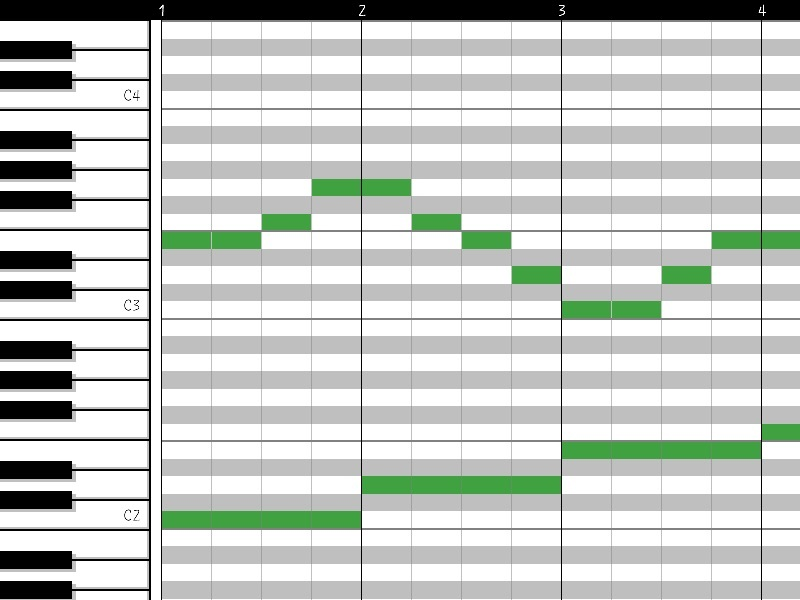
\includegraphics[height=40mm, width=50mm]{z_images/2_midi/exemple_midi_piano.jpg}
	\caption{Exemple évènements avec durée}
\end{figure}
\newpage
Chaque évènement MIDI rassemble un ensemble d’informations sur la hauteur, la durée, le volume, etc… :
\begin{figure}[h]
	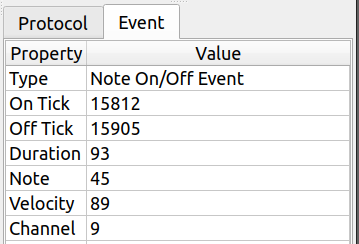
\includegraphics[height=40mm, width=50mm]{z_images/2_midi/representation_numerique_1.png}
	\caption{Critère pour un évènement}
\end{figure}\\
Pour la batterie, les évènements sont considérés sans durée, nous ignorerons donc les offsets (« Off Event »), les « Off Tick » et les « Duration ». Le channel ne nous sera pas utile non-plus.
\textit{Ici, définir Tick et channel.}
Voici un exemple de piano-roll midi pour la batterie :
\begin{figure}[h]
	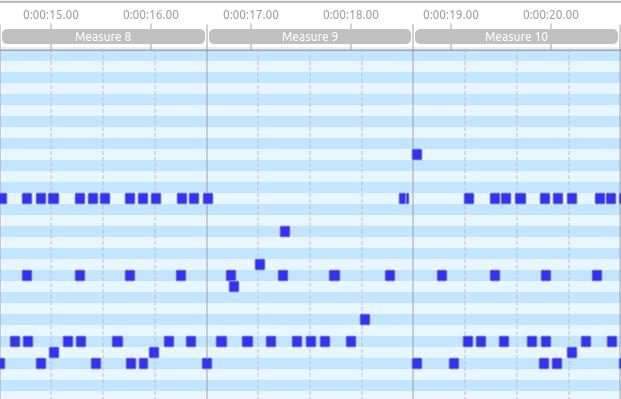
\includegraphics[height=40mm, width=50mm]{z_images/2_midi/representation_numerique_0.png}
	\caption{Exemple évènements sans durée}
\end{figure}\\
On observe que toutes les durées sont identiques.
\subsubsection{La grammaire pondérée}
Système de rythmes préférés.
\subsubsection{Le parsing}
Le parsing du midi donné en input crée une représentation symbolique sous forme d’arbre de rythme.\\
Ici $\Rightarrow$ exemple avec :\\
3bars\_fill\_groove-016.mid $\Rightarrow$ arbre\\
\subsubsection{La séparation des voix}
Plusieurs écritures sont possibles pour un même rythme :
\begin{figure}[h]
	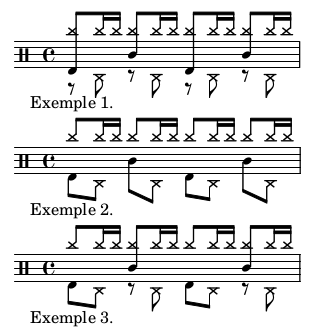
\includegraphics[height=65mm, width=60mm]{z_images/1_description_notation/separation/0_exemples_separation.png}
	\caption{Séparation des voix}
\end{figure}\\
Sur la figure 3.4, il faudra faire un choix entre les exemples 1, 2 et 3 qui sont trois façon d’écrire la même chose. Ce choix se fera en fonction de la lisibilité, de quelles instruments auront des phrasés plus ou moins chargé et/ou variés, auquel cas on les mettra dans une seule voix afin de ne pas charger la partition, etc.
Ainsi l’arbre syntaxique de départ sera divisé en autant d’instruments qui le constituent et les voix seront regroupées de manière cohérentes.
\subsubsection{Les règles de réécriture}
Ici, description basique des règles de réécriture 
\section{Les contributions}
\subsection{Notations, systèmes et réécriture}
\subsubsection{La notation de la batterie}
\textit{Les 3 parties d’une note en général :}
\begin{itemize}
	\item durée
	\item hampe
	\item tête de note (peut aussi indiquer la durée mais en batterie on évitera les blanches, etc.)
\end{itemize}
source : \url{https://fr.wikipedia.org/wiki/Note_de_musique}

\subsubsection{Hauteurs et têtes de notes pour la batterie}
Pour la transcriptions, nous proposons de choisir la base Agostini. La caisse claire centrale sur la portée est aussi centrale sur la batterie est elle est un élément qui conditionne la position des jambes (écart entre les pédales, etc.) ainsi que l’organisation des éléments en hauteur (toms, cymbales, etc.).
On pensera en terme de symétrie la répartition des éléments par rapport au point central que constitue la caisse claire.\\
Cette symétrie s’opère en trois dimensions :
\begin{itemize}
	\item Les hauteurs en terme de fréquences ;
	\item La hauteur physique des éléments :\\
	Du bas vers le haut : pédales, toms et caisse, cymbales
	\item L’ergonomie, qui hiérarchise l’importance des éléments sur la portée (caisse claire au centre, hh-pied et ride sont aux deux extrémités).
\end{itemize}
\begin{figure}[h]
	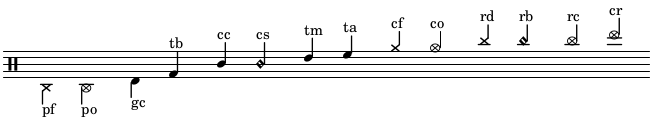
\includegraphics[height=30mm, width=155mm]{z_images/1_description_notation/notes.png}
	\caption{Hauteur et têtes de notes}
\end{figure}
\subsubsection{Les nuances}
\begin{figure}[h]
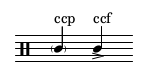
\includegraphics[height=20mm, width=35mm]{z_images/1_description_notation/nuances.png}
\caption{Nuances}
\end{figure}
Bien expliquer les accents, remplacer p et f par g et a\\
$\Rightarrow$ nuance VS articulation\

\subsubsection{Les durées}
Basé sur \cite{jacquemard:hal-01134096} et sur \cite{jacquemard:hal-01403982}\\
Pour la plupart des instruments mélodiques, la liaison et le point sont les deux seules possibilités en cas d’équivalence rythmique pour des notes dont la durée de l’une à l’autre est ininterrompue. Mais puisque les durées des notes n’ont pas d’importance en batterie, l’usage des silences pour combler la distance rythmique entre deux notes devient possible.\\
Ceci pris en compte, et étant donné que les indications de durée dans les têtes de notes ne sont pas pratique en batterie (les symboles « x » des cymbales ne
peuvent pas porter d’indication de durée dans la tête de notes\footnote{Certains logiciels le permettent mais leur lecture reste peu aisée}), l’écriture à l’aide de silences sera privilégiée comme indication de durée sauf dans les cas où cela reste impossible. Ce choix à pour but de n’avoir qu’une manière d’écrire toutes notes, que leurs têtes de notes soit modifiées ou non.\\\\
\textit{Exemple blanche vs noire + soupir}\\

Les cymbales-crash et les ouvertures de charley constituent les seusl cas qui excluent cette option. Le charley car ses ouvertures/fermetures sont presque toujours quantifiées et les cymbales-crash car elles peuvent être arrêtées à la main de manière quantifié aussi mais ce cas est très rare, nous allons donc nous concentrer sur les ouvertures de charley et considérer les crashs comme des événements sans durée.\\
Les fermetures du charley sont notées soit par un silence (correspondant à une fermeture de la pédale), soit par un écrasement de l’ouverture par un autre coup de charley fermé, au pied ou à la main.
\begin{figure}[h]
	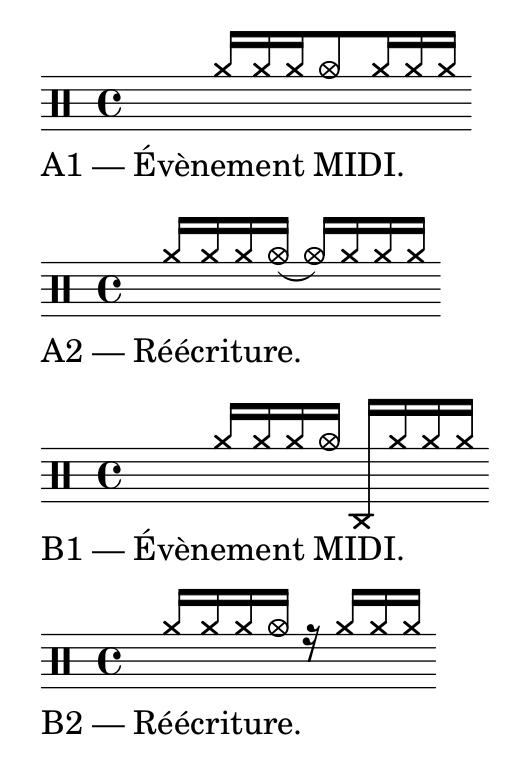
\includegraphics[height=80mm, width=60mm]{z_images/reecriture/exemples_charley_1.png}
	\caption{Durées}
\end{figure} 
\subsection*{La représentation numérique de la batterie}
\subsubsection{Les pitchs}
\begin{table}[h]
	\centering
	\begin{tabular}{|c|c|c|} \hline
		Codes & Instruments & Pitchs \\ \hline
		cf & charley-main-fermé & 22, 42 \\
		co & charley-main-ouvert & 26 \\
		pf & charley-pied-fermé & 44 \\
		rd & ride & 51 \\
		rb & ride-cloche (bell) & 53 \\
		rc & ride-crash & 59 \\
		cr & crash & 55 \\
		cc & caisse-claire & 38, 40 \\
		cs & cross-stick & 37 \\
		ta & tom-alto & 48, 50 \\
		tm & tom-medium & 45, 47 \\
		tb & tom-basse & 43, 58 \\
		gc & grosse-caisse & 36 \\ \hline
	\end{tabular}
	\caption{Pitchs et instruments}
	%	\label{tab:exemple}
\end{table}
Pas de charley pied ouvert…
\subsubsection{La vélocité}
\begin{table}[h]
	\centering
	\begin{tabular}{|c|c|c|c|} \hline
		Codes & Instruments & Pitchs & Vélocité \\ \hline
		cop & charley-main-ouvert & 46 & ? \\ \hline
	\end{tabular}
	\caption{Vélocité et nuances}
\end{table}
Nous ne prendrons en compte la vélocité que pour la cc, les toms et les cymbales jouées aux mains. Les nuances de grosse caisse et charley aux pieds sont le plus souvent insignifiantes, elles ne sont marquées sur le figure qu’à titre indicatif.
Si la vélocité est en dessous de 40, il s’agit de ghost-notes : la tête de note devra être entouré de parenthèses et le suffixe \textit{p (piano)} devra être ajouté au codes de l’instrument. (Voir ccp ci-dessus.)
Si la vélocité est au dessus de 90, il s’agit de notes accentuées : le symbole « > » et le suffixe \textit{f (forte)} devra être ajouté au codes de l’instrument. (Voir ccf ci-dessus.)
Lorsque la vélocité va de 40 à 89, on considèrera le volume comme normal et aucun symbole supplémentaire ne sera ajouté à la note.\\\\

\subsubsection{Les dilemmes}
Le charley de pitch 46 est considéré comme le charley ouvert joué à la main sur le haut de la cymbale mais souvent, ça correspond au geste « tranche-olive » de la baguette lorsque le batteur accentue avec la tranche et joue moins fort avec l’olive sur le plat de la cymbale. Je vais dans un premier temps considérer le pitch comme \textbf{charley-main-ouvert-piano} (ghost-note)
\newpage
\subsubsection{Représentations en arbres}
Voici une représentation de la \textit{partition 3} en arbre de rythme avec les codes de chaque instrument :\\\\
\Tree[ [ [rd\\gc ][ [rd\\pf ][rd ]]]
[ [rd\\cc ][ [rd\\pf ][rd ]]]
[ [rd\\gc ][ [rd\\pf ][rd ]]]
[ [rd\\cc ][ [rd\\pf ][rd ]]] ]\\\\\\
Ci-dessous, le même arbre dont les codes des instruments sont remplacés par leurs données midi respectives :\\\\
\Tree[ [ [51\\36 ][ [51\\44 ][51 ]]]
[ [51\\38 ][ [51\\44 ][51 ]]]
[ [51\\36 ][ [51\\44 ][51 ]]]
[ [51\\38 ][ [51\\44 ][51 ]]] ]\\\\\\
Cet arbre représente un rythme unique dont les possiblités de notation sur une partition sont théoriquement multiples.(Voir \textit{partition 3}).
\subsection*{Les systèmes}
\subsubsection{Définition}

Un système est la combinaison d’un ou plusieurs éléments qui jouent un rythme en boucle (motif) et d’un autre élément qui joue un texte rythmique variable mais respectant les règles propre au système (gamme).\\

Système = motif + gamme/texte\\
motif = rythmes coordonnés joués avec 2 ou 3 membres en boucle (reparti sur 1 ou 2 voix)\\
gamme/texte = rythme irrégulier joué avec un seul membre sur le motif (Réparti sur 1 voix). La gamme d’un système considère l’ensemble des combinaisons que le batteur pourrait rencontrer en interprétant un texte rythmique à l’aide du système.\\

Nous partirons de propositions génériques de systèmes (environs trois systèmes dans différents styles de batterie) que nous tenterons de détecter dans le jeu de données groove.\\

Quatre systèmes standards :
\begin{itemize}
	\item binaire
	\item ternaire (shuffle, afro, rock)
	\item jazz
	\item afro-cubain\\
\end{itemize}

Nous travaillerons aussi sur la détection de répétitions sur plusieurs mesures afin de pouvoir corriger des erreurs sur une des mesures qui aurait dû être identique aux autres mais qui présente des différences.

\subsubsection{Utilité}
\begin{itemize}
	\item Séparation des voix
	\item Définir une métrique
	\item Conditionner des règles spécifiques de réécriture
\end{itemize}

Créer un ensemble de systèmes :
\begin{itemize}
	\item 4/4 binaire FAIT
	\item jazz vs ternaire(12/8) EN COURS…
	\item afro-cubain
	\item Tout transcrire avec lilypond et en arbres d’analyse syntaxique.
	\item Créer les arbres de voix séparées.
	\item Écrire les règles de réécriture.
	\item Créer les arbres de voix séparées simplifiés (rewriting).\\	
\end{itemize}

Pour la \textbf{séparation des voix} et la \textbf{définition des métriques}, nous nous intéresserons principalement à la partie \textit{motif} des systèmes qui seront présentés. La partie \textit{texte} nous intéressera plus pour les \textbf{combinaisons de réécritures}.
\newpage
\subsubsection{Pour la séparation des voix}
\textbf{Motif 4-4 binaire}\\\\
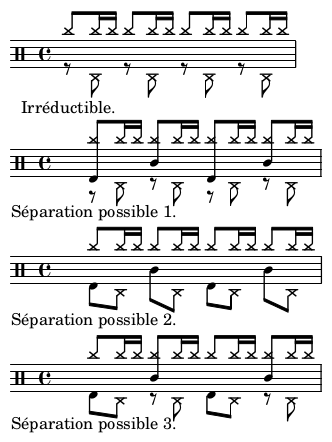
\includegraphics[height=60mm, width=40mm]{z_images/1_description_notation/separation/1_separation_4-4_binaire.png}\\\\
Ici, le système est construit sur un modèle rock en 4/4 : after-beat sur les 2 et 4 avec un choix de répartition des cymbales type fast-jazz. Le système est constitué par défaut du motif ride/ch-pf/cc et d’un texte joué à la grosse-caisse. La troisième séparation proposée est privilégiée car elle répartit selon 2 voix, une voix pour les mains (ride + cc) et une voix pour les pieds (ch-pf + gc). Ce choix paraît plus équilibré car deux instruments sont utilisés par voix et plus logique pour le lecteur puisque les mains sont en haut et les pieds en bas.\\
%D’autres choix d’écriture auraient été possibles :
%\begin{itemize}
%	\item Toutes les hampes en haut ;
%	\item Combinaison motif 1 et 2 en donnant 2 directions aux hampes de la cc).\\
%\end{itemize}

\textbf{Motif 4-4 jazz}\\\\
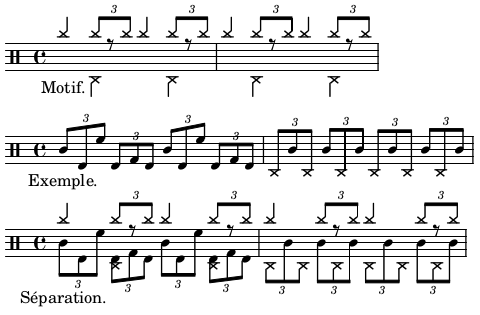
\includegraphics[height=45mm, width=60mm]{z_images/1_description_notation/separation/2_separation_4-4_jazz.png}\\\\
Dans la plupart des méthodes, le charley n’est pas écrit car considéré comme évident en jazz traditionnel. Ce qui facilite grandement l’écriture : la ride et les crash sur la voix du haut et le reste sur la voix du bas. Ici, le partie prit et de tout écrire. Dans l’exemple ci-dessus, les mesures 1 et 2 combinées avec le \textit{motif} de la première ligne, sont des cas typiques de la batterie jazz. Tout mettre sur la voix haute serait surchargé. De plus, la grosse caisse entre très souvent dans le flot des combinaisons de toms et de caisse claire et son écriture séparée serait inutilement compliquée et peu intuitive pour le lecteur. Le choix de séparation sera donc de laisser les cymbales en haut et toms, caisse-claire, grosse-caisse et pédale de charley en bas.
\newpage

\textbf{Système 4-4 afro-cubain}\\\\
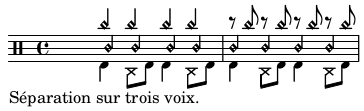
\includegraphics[height=25mm, width=80mm]{z_images/1_description_notation/separation/3_separation_afro-cubain.png}\\\\

\subsubsection{Pour la reconnaissance de la métrique}
\textit{\textbf{12/8 vs 4/4 ternaire}}\\\\
\textbf{Motif 12/8}\\\\
%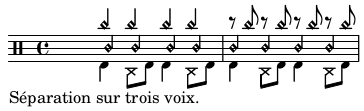
\includegraphics[height=30mm, width=100mm]{z_images/1_description_notation/separation/separation_2.png}\\\\

\subsubsection{Pour les règles de réécriture}
Les textes qui accompagnent les motifs étayent toutes les combinaisons d’un systèmes. 
\newpage

%\subsubsection{Construction des systèmes pour les expérimentations}
\subsubsection{La réécriture des évènements MIDI pour la batterie}



\textbf{Exemples à écrire en arbre :}\\
\begin{itemize}
	\item 
	SI (pas pf) ET (note sur un temps suivie de note en l’air) :\\
	$\Rightarrow$ (Temps1 : Note pertinente) + (Temps2 : Silence pertinent + Note pertinente.)\\
	\item
	Si (po ou co) déborde sur le temps suivant :\\
	$\Rightarrow$ Liaison car marchera dans tous les cas même la où le point ne marchera pas (voir A2).\\
	\item
	Une blanche sera écrite noir + soupir.\\\\
\end{itemize}
\subsubsection{Les régles de réécriture}
~~\\
\Tree[.$\frac{2}{8}$ [.x ][.tie ]]\Tree[.2/8 [.x ]]\\\\\\
\Tree[.1/4 [.x ][.tie ]]\Tree[.1/4 [.x ][.r ]]\\\\\\

\section{Conclusion}
Bilan sur les différentes méthodes employées et la contribution que cela représente.